\chapter{Results}
\section{Experiment 1}
\paragraph{}
Our testing results, presented in Table \ref{tbl:ex1}, demonstrate that both classical feed-forward networks and deep learning configurations are capable of achieving near-perfect classification on the testing dataset with a reasonably sized neural network. The deep learning network achieved an exceptional performance, converging in only 20 epochs with a final classification accuracy of 99\%. In comparison, the feed-forward network reached an accuracy of 98\%  but required nearly all the allotted epochs to reach this level of performance. While it is possible that the feed-forward network could match the deep learning network's performance with additional training epochs, resource constraints precluded this, and such an extension was unnecessary for the purposes of Experiment 1.
\paragraph{}
These findings suggest the presence of an underlying pattern within the Arabic numeral system that can be effectively learned by both approaches. Furthermore, as illustrated in Figure \ref{fig:ex1loss}, the deep learning configuration demonstrated substantially faster convergence, underscoring the efficiency of convolutional layers in feature extraction and their role in expediting convergence in the training process.
\paragraph{}
It is important to note that throughout this experiment, the deep learning component accounted for the majority of the runtime. This is acceptable, as our primary goal is to demonstrate the benefit of feature extraction on classification performance, rather than to assess computational efficiency. While deep learning may be outclassed for a relatively simple problem like this, it becomes a more viable option for more complex tasks. In such cases, feature extraction could offer a significant advantage, as the large size of a feed-forward-only network may become impractical.


\begin{center}
	\begin{figure}[H]
		\centering
		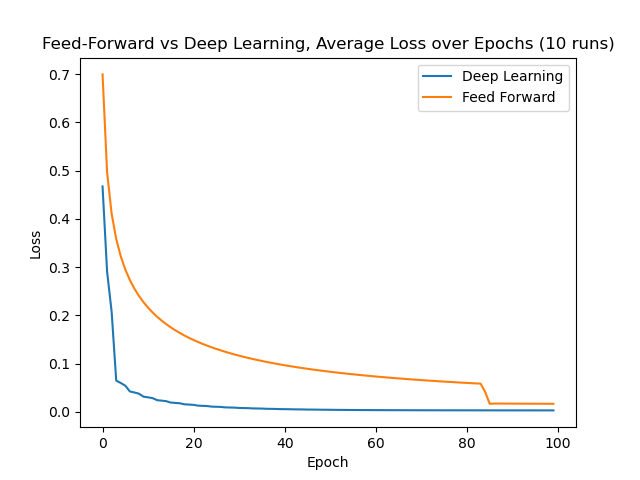
\includegraphics[width=\textwidth]{screenshot001}
		\caption{Experiment 1 Feed-Forward vs Deep Learning, average loss while training.}
		\label{fig:ex1loss}
	\end{figure}
\end{center}

\begin{table}[H]
	\centering
	\begin{tabular}{|c|c|c|c|}
		\hline
		Test & Correct & Incorrect & Accuracy (\%) \\
		\hline
		Feed-Forward & 9800 & 199 & 98\\
		\hline
		Deep Learning & 9898 & 101 & 99\\
		\hline
	\end{tabular}
	\caption{Experiment 1 results on testing dataset. (Averaged over 10 runs)}
	\label{tbl:ex1}
\end{table}

\section{Experiment 2}
\paragraph{}
In Experiment 2, the benefits of deep learning are evident, as shown in Table \ref{tbl:ex2}. Despite the significantly reduced size of the classification network, the deep learning configuration maintains the 99\% accuracy achieved in Experiment 1. In contrast, the feed-forward network's performance declines, now achieving only 96\% accuracy. Notably, the deep learning network still converges within 20 epochs, similar to Experiment 1. While the feed-forward network roughly converges within 40 epochs and continues to improve throughout the remainder of the run, it never reaches the peak classification accuracy observed in Experiment 1.
\paragraph{}
It could certainly be argued that the reduced size of the feed-forward network is the primary cause of the observed decrease in performance. However, this only serves to highlight the value of feature extraction. Feature extraction allows for the provision of more information-dense data to the classification network, and, as clearly demonstrated in this experiment, it significantly enhances overall performance. While allowing the feed-forward network more training time might help improve its results, the benefit of feature extraction in the deep learning configuration remains evident.

\begin{center}
	\begin{figure}[H]
		\centering
		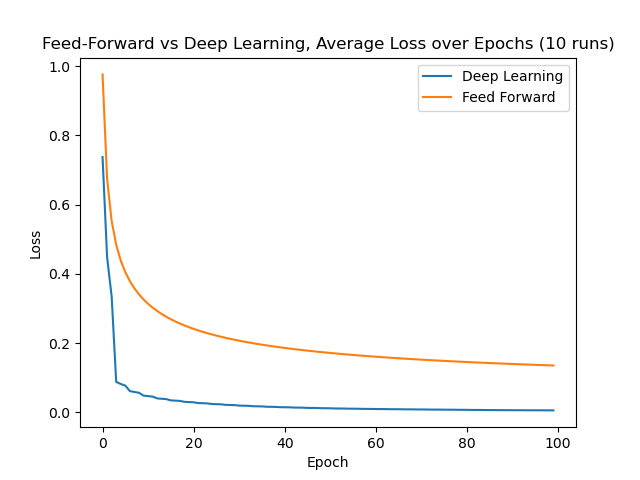
\includegraphics[width=\textwidth]{screenshot002}
		\caption{Experiment 2 Feed-Forward vs Deep Learning, average loss while training.}
		\label{fig:ex2loss}
	\end{figure}
\end{center}

\begin{table}[H]
	\centering
	\begin{tabular}{|c|c|c|c|}
		\hline
		Test & Correct & Incorrect & Accuracy (\%) \\
		\hline
		Feed-Forward & 9588 & 411 & 96\\
		\hline
		Deep Learning & 9887 & 112 & 99\\
		\hline
	\end{tabular}
	\caption{Experiment 2 results on testing dataset. (Averaged over 10 runs)}
	\label{tbl:ex2}
\end{table}